\documentclass[12pt,a4paper]{article}
\title{Experiment 15: Virtualisation Environment}
\author{Aarya R Shankar} 
\date{May 14, 2017}
\usepackage{hyperref}
\hypersetup{
    colorlinks=true,
    urlcolor=blue,
}
\usepackage{graphicx}
\begin{document}
\maketitle
\section{Aim}
 
Virtualisation environment (e.g., xen, kqemu, virtualbox or lguest) to test an applications, new kernels and isolate applications. It could also be used to expose students to other alternate OSs like *BSD

\section{Procedure}

Sometimes we may want to install a new OS, but already 4 partitions are made in the disks, or we may want to test a software application, which may or may not harm your computer, etc. For these purposes, we install and use a virtualisation environment in our present operating system, and it will act as a separate machine. Hence, a single machine can act as different machines.\\
There are several virtualisation softwares available for this purpose. Here, we'll be using KVM.\\
KVM (for Kernel-based Virtual Machine) is a full virtualization solution for Linux on x86 hardware containing virtualization extensions (Intel VT or AMD-V). It consists of a loadable kernel module, kvm.ko, that provides the core virtualization infrastructure and a processor specific module, kvm-intel.ko or kvm-amd.ko.\\
Note: It is preferred to use 64 bit kernel system as the host machine, as they can support 32 bit as well as 64 bit. In addition to that, 64 bit does not restrict RAM usage of the OS in the virtual environment (guest OS) to 2 GB, which will inevitably decrease its speed.\\
To know if our kernel is 64 bit, execute:\\
\texttt{\ uname -a}\\
Expected output: \texttt{\ x86\texttt{\_}64 in the output}\\
To know if our processor supports 64-bit instructions, execute:\\
\texttt{\ egrep -c ' lm ' /proc/cpuinfo}\\
Expected output: \texttt{\ 1 or higher}\\
To know if ou processor support hardware virtualisation, execute:\\
\texttt{\ egrep -c '(vmx|svm)' /proc/cpuinfo}\\
Expected output: \texttt{\ 1 or higher}\\
\newline
Assuming that all the outputs are as expected, let us now install KVM, by executing:\\
\newline
\texttt{\ sudo apt-get install qemu-kvm libvirt-bin bridge-utils}\\
\newline
To install the GUI tool, execute: (Not necessary)\\
\newline
\texttt{\ sudo apt-get install virt-manager}\\
\newline
If we are not a root user and we want to launch VMs without root privileges, log out and log in after executing:\\
\newline
\texttt{\ sudo adduser username libvirt}\\
\newline
Now run:\\
\newline
\texttt{\ virsh -c qemu:///system list}\\
\newline
If the output is an empty set of VMs, it means that the KVM is installed successfully.\\
\begin{figure}[h]
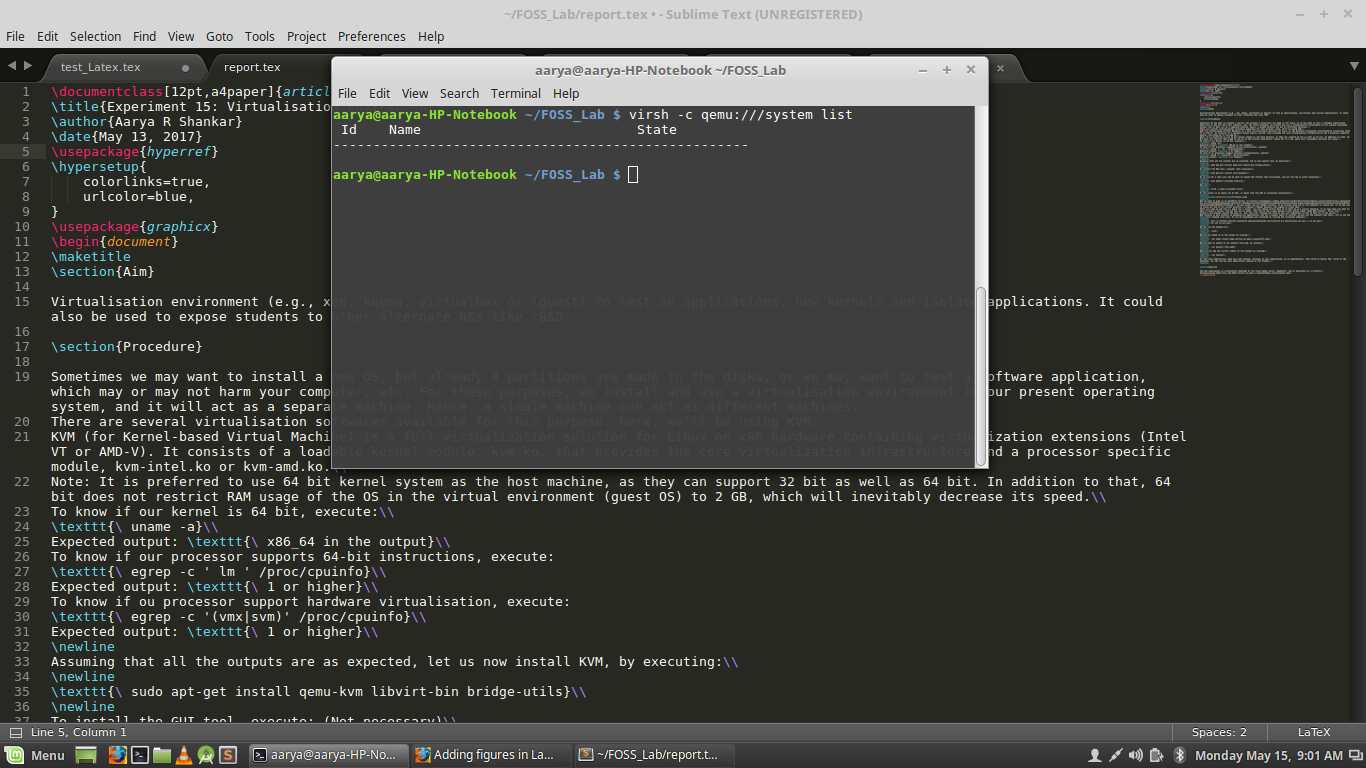
\includegraphics[width=\textwidth]{KVMSetUpSuccess}
\centering
\end{figure}
\newline
Now we have successfully set up the KVM, we need to create a hard disk image, which are of 2 types: raw and qcow2.\\
A raw disk image file is an exact bit-for-bit copy of the hard drive, that is, a complete copy of all of the data stored on the source drive. It provides the lease I/O overhead, but it causes lots of space-wastage as the unused space of the guest OS can't be used by the host OS.\\
A qcow2 disk image only allocates the physical space needed by actual data stored to the virtual disk, ie, entire virtual disk size doesn’t need to be allocated on the hard drive when it’s created. Due to this, the space usage is optimal, but this type has a processing, as well as I/O overhead, due to which its performance will not be as good as the former.\\
\newline
To create a hard disk image of 10 GB in raw format, execute:\\
\newline
\texttt{\ qemu-img create -f raw firstvirtimg.img 10G}\\
\newline
To create a hard disk image of 10 GB in qcow2 format, execute\\
\newline
\texttt{\ qemu-img create -f qcow2 firstvirtimg.qcow2 10G}\\
\newline
To verify the image, execute:\\
\newline
\texttt{\ ls -lh firstvirtimg.img}\\
\newline
To resize the disk image (raw or qcow2 type) to 12GB, execute:\\
\newline
\texttt{\ qemu-img resize firstvirtimg.img +2G }\\
\newline
Now execute:\\
\newline
\texttt{\ ls -lh firstvirtimg.img }\\
\newline
We can see that the size of the disk image increased by 2GB.\\
To convert a qcow image 'test.img' to a raw 'test.raw' file, run:\\
\newline
\texttt{\ qemu-img convert test.img -O raw test.raw}\\
\newline
To convert a raw 'test.img' file to a qcow image 'test.qcow', run:\\
\newline
\texttt{\ qemu-img convert test.img -O qcow2 test.qcow2}\\
\newline
To verify the image, execute:
\newline
\texttt{\ ls -lh firstvirtimg.img }
\newline
To resize the disk image (raw or qcow2 type) to 12GB, execute:\\
\newline
\texttt{\ qemu-img resize firstvirtimg.img +2G }\\
\newline
Sometimes we need to revert a change we made in the guest system. For this, we make a backup image or a storage image and a overlay image to keep the changes we make to the storage image. So when we want to reverse the last change, we only need to create an overlay image of the current storage image. To create an overlay image, execute:\\
\newline
\texttt{\ qemu-img create -f qcow2 -b firstvirtimg.qcow2 firstvirtimg.ovl}\\
Now we can run our QEMU VM as usual by using the overlay image so as to save the new changes in it, by executing the command:\\
\newline
\texttt{\ qemu-system-i386 -enable-kvm firstvirtimg.ovl}\\
\newline
To run Arch Linux without a virtual hard drive in the virtualised system, execute:\\
\texttt{kvm -m 2048 -cdrom archlinux-2017.02.01-dual.iso -boot d  &}\\
\newline
Here \texttt{\ kvm} is a script which executes \texttt{\ qemu-system-x86\texttt{\_}64 -enable-kvm}\\
\texttt{\ -enable-kvm} enables kvm extensions\\
\texttt{\ -m num} sets the RAM of the virtual system to num megabytes\\
\texttt{\ -cdrom} uses the iso file as CD-ROM image\\
\texttt{\ -boot d} specifies CD-ROM drive (indicated by d) as the first one in boot order.\\
\newline
The KVM has successfully run the arch linux iso file. It is also possible to install and run any other operating system or application in the KVM.\\
\newline
\section{Result}
The KVM is successfully set up. The virtual machine has been successfully booted with the iso file of Arch Linux.
\end{document}
